\epigraph{%
  ``\elide\ This begs the question: if a patient had reliable control
  over their eye gaze, why would one aim to facilitate communication with that
  patient via a BCI? It would be far simpler and more efficient to use an
  eye-tracking system.
  And even if a BCI were the preferred or only available option for some reason,
  designs requiring eye gaze control could not be used
  by patients with severe motor impairment, as these patients
  cannot direct their gaze.
  Because these are the patients who have the greatest need for BCIs, it is
  important that accurate gaze-independent BCIs exist.''
}{%
  \textcite{Egan2017}
}
\todohsm{move introduction of paper to paper}

\emph{Parts of Sections~\ref{sec:gaze-dependence} and~\ref{sec:gaze-independence}
have been published by \textcite{VanDenKerchove2024}.}

\todo{spatially vs temporally organized interfaces}
\todo{talk about covert shifts in spatial attention alpha}

\section{The gaze-dependence problem}%
\label{sec:gaze-dependence}

\todo{define eye motor issues}

\todo{Algemeen: in begin uitleggen dat de ziektes er niet veel toe doen en dat
het gaat over verlamde personen, verlies van spierkracht en coördinatie en dus
gehinded in communicatie, helemaal in begin van chapter 1 duidelijk maken dat
het om deze patiënten gaat}
One of the goals of brain-computer interfacing is establishing a communication
channel that does not rely on speech or muscular activity~\cite{Naci2012,Chaudhary2016},
which in turn can provide solutions to paralyzed individuals.
In the strictest interpretation, this also means that an interface should not
rely on the control of eye muscles used to redirect the gaze or for blinking.
\todo{patients suffering paralysis due to damage to the CNS (stroke, spinal
chord injury, tbi) or neurodegenerative diseases}

In fact, many patients in the \ac{bci} target population suffer to some extent
from eye motor disability, requiring \ac{bci}s adapted to their condition.
Table~\ref{tab:incidence} reports the relatively high frequencies of
eye motor problems, which can range from minor (nystagmus
\footnote{%
Involuntary, rhythmic, and repetitive eye movements recognizable by their
consistent directionality (horizontal, vertical, or rotational).
}, other eye tremors
\footnote{%
These can include square-wave jerks, saccadic intrusions, microtremors, or
microsaccades while resting or fixating the gaze.
}, gaze fixation fatigue or discomfort, \ldots), to severe (partial ophtalmoplegia
\footnote{%
Weakness or limited paralysis of one or more of the muscles that control eye
movement, leading to restricted eye motion, but not complete paralysis.
Often, a specific movement direction (up-down, left-right) is preserved.
}, involuntary movements, impaired pursuit, \ldots), and even complete
ophtalmoplegia\footnote{Full eye movement paralysis.} or eye motor paresis.
This not only has an effect on vision and coordination but also
on their ability to operate a visual \ac{bci}.

\begin{table}[h]
  \sffamily
  \footnotesize
	\centering
	\begin{tabular}{@{}l|rrrrr|r@{}}
    & \bfseries \acs{als} & \bfseries \acs{ms}   & \bfseries Stroke &\bfseries\acs{dmd} &\bfseries \acs{sma} &\bfseries \acs{lis} \\ \hline
		\bfseries Minor    & 50\% & 31\% & 40-70\% & + & - &      \\
		\bfseries Severe   & 33\% & 3\%  & +       & - & - & 98\% \\
		\bfseries Complete & 17\% & -    & +       & - & - & 2\%  \\
	\end{tabular}
	\caption{Incidence of eye motor impairment in selected \ac{bci} target
    patient populations. (\acs{als}: \acl{als}, \acs{ms}: \acl{ms}, \acs{dmd}:
    \acl{dmd}, \acs{sma}: \acl{sma}, \acs{lis}: \acl{lis}).
    $+$: frequent, $-$: infrequent.}
    \label{tab:incidence}
\end{table}
\todo{include FA}
\todo{cite Abnormal Oculomotor Functions in Amyotrophic Lateral Sclerosis 10.3988/jcn.2018.14.4.464}
\todo{cite Neuro-Ophthalmologic Manifestations of Amyotrophic Lateral Sclerosis}

\todo{
14] Fazzi E, Signorini SG, Piana RL, et al. Neuro-ophthalmo-
logical disorders in cerebral palsy: ophthalmological, oculo-
motor, and visual aspects. Dev Med Child Neurol. 2012;54:
730–736.
[15] Graber M, Challe G, Alexandre MF, et al. Evaluation of the
visual function of patients with locked-in syndrome: report
of 13 cases. J Fr Ophtalmol. 2016;39:437–440.
[16] Moss HE, McCluskey L, Elman L, et al. Cross-sectional evalu-
ation of clinical neuro-ophthalmic abnormalities in an
amyotrophic lateral sclerosis population. J Neurol Sci. 2012;
314:97–101.
}

Among the most affected patients are stroke patients~\cite{Pollock2011}, mostly
due to brainstem or cerebellar stroke~\cite{Moncayo2009,Bogousslavsky1987}.
\todo{summarize and cite Rowe2019}
These patients might suffer from severe or complete eye motor impairment
from the onset of their condition.
In \ac{als}, a progressive disease, oculomotor issues are also fairly common.
Although eye movement is often cited as one of the longest preserved
capabilities in \ac{als}, \textcite{Guo2022} show that minor issues are still
fairly common,
especially for patients with bulbar onset \ac{als}.
Furthermore, \textcite{Hayashi1991} show that, as these patients progress past
the point of independent breathing, symptoms will eventually also involve
eye muscle paralysis.
Various forms of eye movement abnormalities also occur often and are especially well studied in
\ac{ms}~\cite{Mueri1985,Prasad2010,Castelnovo2016,Serra2018,Polet2020}.
These abnormalities can be minor or severe, seldom progressing to complete
paralysis.
However, \ac{ms} often comes with vision loss, further complicating interaction
with visual \acp{bci}.
\todo{FA}
Patients suffering from other neurodegenerative diseases like
\ac{sma}~\cite{Anagnostou2021} and \ac{dmd}~\cite{Lui2001} are
sometimes also interested in \ac{bci} use, but their eye motor capabilities are
mostly preserved.

\newcommand\fnlis{\footnote{
Multiple definitions of \ac{lis} are encountered in
\ac{bci} and neurological literature.
Some definitions include only tetraplegic patients without eye movements used
for communications.
Others distinguish Complete Locked-in Syndrome (CLIS) with full body paralysis,
including no eye motor control at all, from a \ac{lis} state with some preserved eye
movements or minor motor output.
While some definitions only include patients who suffered stroke or traumatic
brain injury to specific regions in the brain (midbrain, brainstem, or
cerebellum)~\cite{Smith2005},
it can also generally refer to the state of full body paralysis
or loss of muscle tone incurred in neurodegenerative diseases, combined with
the inability to speak, such as occurs in late stage ALS.
In clinical reality, every tetraplegic patient has their own unique set of
preserved capabilities and from a solution-oriented \ac{bci} engineering point
of view, the etiology of the symptoms can be abstracted away.
}}

\newcommand\fnwolpawcrit{\footnote{
\it``The first class consists of people who are truly totally locked-in (e.g.,
due to end-stage ALS or severe cerebral palsy), who have no remaining
useful neuromuscular control of any sort, including no eye movement.
\elide\ This class is very small. \elide\
The second class of potential \ac{bci} users comprises those who retain
a very limited capacity for neuromuscular control. This group includes
people who retain some useful eye movement or enough limb muscle
function to operate a single-switch system. Such control is often slow,
unreliable, or easily fatigued.
This group is much larger than the first.
}}


Together, some of these patients constitute the \ac{lis} patient group, which
forms one of the main \ac{bci} target populations.
In this work, we define \ac{lis} patients as those in a situation of (near)
complete paralysis and difficulties or the inability to communicate without
assistive technology.
This corresponds to classes one and two defined by
\textcite{Wolpaw2006}\fnwolpawcrit.
Additionally, some degree of severe or complete eye motor impairment is usually
necessary to qualify as locked-in\fnlis.
Since this work is concerned with gaze-impaired patients, we will adopt this
interpretation into our definition.
Case study reports~\cite{Patterson1986} show that the population of locked-in
patients with complete eye motor paralysis is very small.
Hence, it would be interesting to focus \ac{bci} development efforts on the
larger population of \ac{lis} patients with severe eye motor impairment that
currently slip through the cracks of the assistive technology offer.
These are the patients whose severe eye motor impairment prevents them from
using eye tracking based solutions.
They currently use their remaining motor control to
communicate by indicating symbols on a letterboard with great effort,
or signal with upwards eye movements or blinks to confirm prompted letters.
They require a caregiver or relative to interpret their signals, and crave
the ability to communicate independently which is crucial to retaining an
acceptable quality of life.
\todo{order of concepts in next two paragraphs can be tweaked}

This leads us to what we call the \emph{gaze-dependence problem in visual
\ac{bci}}:
Traditional visual \ac{bci} scenarios require the user to overtly direct their both
\ac{vsa} and gaze toward the screen target they intend to select.
For our purposes, screen targets are overlaid with non-overlapping, transient
stimuli that evoke \acp{erp} in the \ac{eeg}.
The selected target can be decoded from these \acp{erp}, as is the case for the
oddball paradigm where observing a rare but attended stimulus evokes a P3 \ac{erp}
component.
However, a critical challenge arises when users rely solely or in part on covert
VSA, which involves directing visuospatial attention without corresponding eye gaze.
In these cases, classical solutions often fall short of the widely accepted
80\% target selection accuracy threshold~\cite{Brunner2010,Frenzel2011,Treder2010,RonAngevin2019} deemed necessary for a comfortable user experience~\cite{Neeling2019}, calling for alternative, gaze-independent
solutions.

To summarize: for patients with eye motor impairment, gazing directly at a screen target may
be uncomfortable, impractical, or even impossible.
Hence, assistive devices that rely on eye tracking are often inefficient for
them.
Consequently, while \ac{bci}s hold great promise for these individuals, conventional
gaze-dependent \ac{bci} solutions do not meet their needs due to the absence of gaze
control.
Therefore, the development of decoding strategies that account for covert
VSA becomes crucial in the pursuit of high-performance gaze-independent
\ac{bci}s.

In this work, we will use the term \emph{gaze-independent} meaning
\emph{‘dealing explicitly with the fact that a user cannot control their
gaze.'}
In the context of a visual \ac{bci}, this means that the user's
visuospatial attention and their gaze do not necessarily coincide.



\section{Gaze-independent \ac{bci} paradigms}
\label{sec:gaze-independence}
\todohsm{rename to state of the art in gaze-independent bci. Address more systematically.}

Gaze-independent \ac{erp}-based \ac{bci}s~\cite{Riccio2012, Aloise2012} can be realized in three
ways.
Firstly, active \ac{bci} communication paradigms relying on endogenous activation from the user
do not rely on sensory stimulation.
Examples of this are imagined movement or imagined speech paradigms.
These paradigms can yield very high information transfer
rates~\cite{Willett2021,Metzger2023}, both due to their intuitiveness and the
complexity that can be captured in commands, but often only do so when paired
with invasive recording.
Non-visual reactive paradigms that use e.g. auditory and
somatosensory\todo{cite some}
stimulation do not rely on gaze redirection exist but also result in lower information transfer
rates compared to visual paradigms.
Furthermore, they can suffer from increased mental effort in operation and
user-dependent variability~\cite{Severens2014,Reichert2020b}.
\textcite{Severens2014} showed that the visual Hex-o-Spell~\cite{Treder2010}
outperformed a somatosensory alternative in participants with \ac{als} whose
eye motor capabilities were effectively impaired.

\todo{insert table from riccio in text as numbers, not as table}

This leads us to the second approach, current visual stimulation paradigms can be optimized, e.g. such that
the stimuli are always present in the field of view either overtly~\cite{Acqualagna2013, Won2018,
Lin2018} or covertly~\cite{,Pires2011,Lees2018}. Some noteworthy examples include the GIBS Block Speller~\parencite{Pires2011},
the GeoSpell interface~\parencite{Aloise2012}, and the RSVP
speller~\parencite{Acqualagna2011}.
Non-spatial visual attention (feature attention) can also be exploited, such as
attention to stimulus color, shape or symbol~\cite{Zhang2010,Treder2011,Hwang2015}.
Alternative visual stimulation paradigms can modulate specific \ac{erp} components
that are more sensitive to stimulation in the visual periphery~\cite{Schaeff2012,Xu2022}.
Nevertheless, these methods can suffer too from reduced information
transfer rates~\cite{Chennu2013}.
Furthermore, these systems typically require users to focus on a central fixation point while
selecting peripheral targets.
This entails that they still rely to some extent on
eye motor control, often necessitating central gaze fixation.
\todo{advantages disadvantages rewrite (requires gaze fixation, low itr, not tested with split attention)}

Thirdly, stimuli can be presented in a standard \ac{bci} paradigm, but visuospatial
attention can be decoded separately from gaze direction.
\textcite{Aloise2012} aimed to bridge the performance gap between covert and
overt VSA decoding performance.
They compared classical linear and non-linear \ac{erp} classifiers on a covert
attention oddball \ac{erp} paradigm dataset.
The results revealed no significant performance improvement in covert VSA
decoding for any of the investigated decoders.
More recent work has made advances in decoding lateralized covert
VSA harnessing the N2pc \ac{erp} component~\cite{Thiery2016,Reichert2020b,Wang2022},
decoding covert VSA shifts from spectral content~\cite{Tonin2013}, or hybrid
stimulation paradigms~\cite{Egan2017}.
Since these methods often require a slower stimulation pace than the classical
\ac{erp} \ac{bci} paradigm, gaze-independent decoding in the fast-paced reactive \ac{erp} paradigm
leveraging spatial attention remains underexplored.

\todo{
  Complete with refs from

Fast detection of covert visuospatial
attention using hybrid N2pc and SSVEP
features
}

\section{Problem statement}

\subsection{Objectives}

\todohsm{ move next two paragraphs to introduction, more context than objectives}
Brain-Computer Interfaces (\ac{bci}s) decode brain activity with the aim to establish a direct communication
pathway bypassing speech and other forms of muscular activity. They have raised great hopes for patients
devoid of these abilities, for whom \ac{bci}s can provide a means to communicate or to
control devices.
An effective and proven method is the \ac{eeg}-based visual event-related potential (\ac{erp})-based
oddball interface~\cite{Wolpaw2018,Severens2020}.
Here, targets are shown in short flashes on a computer screen.
Each time the user observes a target, an \ac{erp} is evoked, the presence of which can be
detected in the EEG-signal.
The \ac{erp} consists of multiple components, of which some are modulated by the
attention of the user, specifically the N2 and the P3 component.
Decoding this modulation allows for information transfer controlled by the
user's brain activity, as sketched in Figure~\ref{fig:bci/loop}.
However, visual \ac{bci}s cannot operate efficiently when the user does not direct
their gaze onto the desired target~\cite{Brunner2010, Frenzel2011}.
\todomvh{I am wondering whether goal statements and patient target groups
should be addressed in chapter 1.}

This leads to the often underadressed gaze-dependence paradox: the \ac{bci} target
population consists of patients who suffer from various degrees
of paralysis, or even from Locked-in Syndrome (LiS), the complete loss of muscle
control with preserved consciousness.
While \ac{bci}s are most attractive as a solution for these patients
compared to other assistive technologies like eye-tracking\todomvh{but with eye
control while the previous sentence points are absence of it}., studies often
report bad performance in patient populations precisely due to the lack of adequate eye motor
control, or patients with gaze impairments are excluded.
Different degrees of eye motor impairment can render visual \ac{bci}s
uncomfortable or outright impossible to use.
When operating a visual \ac{bci}, the usual rapid series of forced saccades followed
by fixation is tiring over time, even for healthy control subjects.
A suitable alternative would allow the user to keep their eyes in an at-rest
position of their choice while operating the \ac{bci}.
This points to the need for gaze-independent \ac{bci}s.

The general goal of this PhD is to tackle the gaze-dependence in visual \ac{bci}s.
\todo{refer to ITRs from previous chapter}
Section~\ref{sec:gaze-independence} showed that visual \ac{bci} paradigms form
a good candidate for a performant gaze-independent \ac{bci}.
While the central gaze fixation of most visual gaze-independent paradigms still
relies to some extent on eye motor control, we aim to circumvent this.
We make a distinction here between spatially organized interfaces, where
multiple targets are displayed at the same time at different spatial locations,
and temporally organized interfaces, like Rapid Serial Visual
Presentation\todo{cite},
where targets or small sets of targets are shown consecutively.
Traditionally, spatially organized interfaces have a higher information transfer
rate, but are also more gaze-dependent than temporally organized interfaces.
In such an interface, stimuli can be presented in a standard \ac{bci} paradigm, but
visuospatial attention can be decoded separately from the position of gaze,
which do not necessarily need to coincide.

This leads us to adopt a specific approach: improve the performance of a
spatially organized visual oddball \ac{erp}-based brain
computer interface by using a suited decoding strategy.
Hence, our working hypothesis is as follows:
\todo{rewrite, this is not what we tested in the patient paper after all}
\begin{quote}
	\textit{A spatially organized visual oddball \ac{erp} \ac{bci} with a suited decoder
		can achieve a similar transfer rate in patient
		populations with eye motor deficits than other gaze-independent alternatives
    described in literature.}
\end{quote}

To achieve our goal, we innovate on decoder development and interface design,
and we collect data from healthy control subjects, which allow us to test our decoders.
Finally, the findings of these experiments will be leveraged to develop a \ac{bci}
for patient use, which will be tested in a case-based patient study in which
both performance and user comfort was be evaluated.\todo{was this actually
done?}

This specific hypothesis is embedded within a broader goal of enabling
effective communication for eye-motor impaired \ac{lis} patients.
Ultimately, we wish to design a comfortable interface that allows them to maximally exploit
their residual gaze capabilities, by leveraging a non-invasive, high-\ac{itr}
\ac{bci} on the one hand, and on the other hand improving \ac{erp} decoding performance
in general.

\section{Approach}

\subsection{Interface design}
\todohsm{rename data collection. start with decoder design, second section data collection with experiments}

\todo{mention, free, split, frenzel}
\todo{clear definitions, table from paper}

First, we designed a visual oddball interface that helps us study and adapt
to the effects of eye motor impairment on the \ac{erp}, when using existing state-of-the-art
decoders and on our own proposed decoders.
Using a hexagonal lay-out interface, similar to the visual Hex-o-Spell proposed
\textcite{Treder2010}, we present six flashing circular targets
(without letters or symbols) to the participant while the EEG and
electro-oculogram (EOG) are recorded, as well as eye gaze using eye tracking.
\todo{chosen because gaze-independent optimized and Peters2020}

The interface can be operated in different VSA conditions as illustrated in
Figure~\ref{fig:gaze-vsa}.
\fourpanefig{%
  \figpane{%
    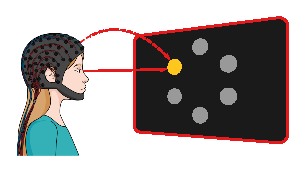
\includegraphics[width=\textwidth]{figures/gaze_independence/attention_overt.eps}
  }{%
    \emph{Overt \ac{vsa}}.
    Gaze and \ac{vsa} coincide on a target.
  }{%
    fig:gaze/vsa/overt
  }
}{%
  \figpane{%
    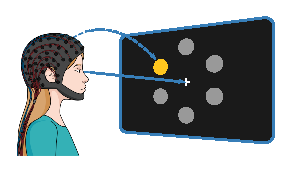
\includegraphics[width=\textwidth]{figures/gaze_independence/attention_covert.eps}
  }{%
    \emph{Covert \ac{vsa}}.
    Gaze rests on the center of the screen, while \ac{vsa} is directed towards a target.
  }{%
    fig:gaze/vsa/covert
  }
}{%
  \figpane{%
    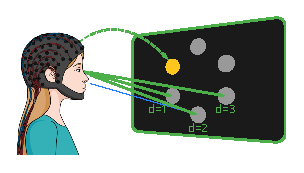
\includegraphics[width=\textwidth]{figures/gaze_independence/attention_split.eps}
  }{%
    \emph{Split \ac{vsa}}.
    \Ac{vsa} is directed towards a target, while the gaze rests on another.
  }{%
    fig:gaze/vsa/split
  }
}{%
  \figpane{%
    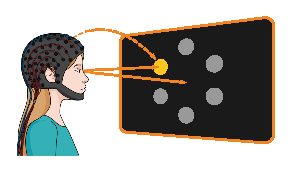
\includegraphics[width=\textwidth]{figures/gaze_independence/attention_free.eps}
  }{%
    \emph{Free \ac{vsa}}.
    The user is free to direct their gaze as they deem most comfortable
    All previous \ac{vsa} conditions are possible.
  }{%
    fig:gaze/vsa/free
  }
}{%
  \Ac{vsa} conditions defined in our hexagonal spatial \ac{erp} paradigm interface.
}{%
  fig:gaze-vsa
}


In the overt case, users gaze at the cued
target they are also mentally attending; in the covert case, users
gaze at the center of the screen while mentally attending to the cued target.
Finally, we introduce a VSA condition that is understudied in the context of
gaze-independent \ac{bci} development: split VSA.
In split VSA, the user mentally focuses on one cued target while gazing at
another (the distractor).
\todomvh{+ "free" condition in Fig. 21.}

The option to dissociate gaze and visuospatial attention will allow us to
investigate the effect of gaze control on \ac{bci} performance.

\subsection{Decoders}

During this PhD, we explored different lines in decoding strategies,
trying to tackle several problems that arise from gaze-independence, such as
the lack or decrease in amplitude of specific \ac{erp} components, and the increased
non-stationarity of the signal.
As mentioned, state-of-the-art decoders have poor performance in covert attention
settings.
The general goal is thus to design a machine learning classifier that represents
the \ac{erp} signal in a specific way, such that it becomes more robust to the problems
occurring in covert attention conditions.

\subsubsection{Regularized spatiotemporal beamforming}
Due to the decreased amplitude of the N1 and P3 components in covert attention
settings~\cite{Treder2010}, the \ac{snr} of
the \ac{erp} is lower than in overt attention settings.
Therefore, a straightforward way to reach satisfactory
gaze-independent decoding performance, might be by increasing overall \ac{erp}
decoding performance. A more accurate classifier could yield relative
improvements in those settings where performance is not yet near the achievable
maximum.\todomvh{?? how to find out what is the maximum?}

Therefore, we have improved upon an in-house developed, state-of-the art \ac{erp}
decoder, the spatiotemporal beamformer~\cite{Wittevrongel2016}, by reformulating
this classifier as a linear discrimination problem and
imposing regularizing constraints by structuring the noise covariance matrix
(STBF-struct).
Furthermore, these regularizing constraints impose temporal stationarity on
the background noise, yielding insights for our next\todomvh{next? more specificaly?}
efforts to cope with the non-stationarity of the P3 signal component.
\todofc{conclue with something like "this approach has been published in ... and
will be described in chapter XXX}

\subsubsection{Classifier-based Latency Estimation with Woody iterations}

P3 latency generally falls between 350ms and 600ms~\cite{Luck2014}, but this
value is heavily dependent on the subject and the task, and can vary from trial
to trial~\cite{Ouyang2017}.
The work of \cite{Arico2014} illustrates that the variation in single-trial P3
latencies is important in gaze-independent decoding and has been hampering covert
VSA decoding performance.
In this work we aim to reprise their hypothesis stating that jitter compensation improves
covert VSA performance and extend it by developing a decoder and evaluating it
in a broader range of gaze-independent settings, including split VSA.

\todo{check overlap}

Literature shows that better covert attention performance can be achieved by
counteracting the non-stationarity of the P3 \ac{erp} component in covert
attention settings~\cite{Arico2014}.
This can be done by estimating the latency of each single-trial \ac{erp} and aligning
the P3 peaks to all fall at the same moment.
The resulting aligned data and the set of latencies can then be used to train a
classifier that is more robust to jitter.

Existing latency estimation methods are either not applicable to the
classification problem of labeling unseen data, or are not robust enough to
deal with the low \ac{snr} of the \ac{erp}.
Classifier-based Latency Estimation (CBLE)~\cite{Mowla2017} is a technique that can leverage
\ac{erp} latency estimation in a decoding setting, but our results show that it
yields no improvement in gaze-independent settings.
We improved upon this technique and extended it to a probabilistic, iterative
method named Classifier-based Latency Estimation with Woody iterations (wCBLE).
\todo{conclue with something like "this approach has been published in ... and
will be described in chapter XXX}

\subsubsection{Tensor discriminant analysis}
\todo{todo}

\subsection{Experiments}

\subsubsection{Healthy control study}
In a first series of experiments, we recorded data with this interface from healthy participants.
The goal of these experiments is to benchmark
gaze-independent \ac{erp} decoding algorithms.
We denote this dataset as the Covert Visuospatial Attention \ac{erp} dataset
(CVSA-\ac{erp})
This study was approved by the Ethics Commission of University Hospital Leuven
(S62547).
To simulate the dissociation between the eye gaze (visual attention) and the
intended target (mental attention) which could occur in patients with hampered eye
motor control, healthy participants are cued to operate the \ac{bci} in specific
\ac{vsa} conditions.
\todofc{conclue with something like "this approach has been published in ...
and will be described in chapter XXX}

\subsubsection{Patient case study}
\todofc{conclue with something like "this approach has been published in ...
and will be described in chapter XXX}

\todo{todo}
\todo{mention multi-center patient study case studies in cooperation
After data collection from healthy participants and decoder development, we
will carry out a patient study using a similar interface.
The goal of the patient study is to evaluate the influence of eye motor
deficits in patient populations on existing state-of-the-art decoders and on
our proposed decoding methods.
}
\todo{update with current results}

\todo{refer to chapters}
